\newpage

\renewcommand{\thesubsection}{\textcolor{red}{\Roman{section}.\arabic{subsection}}}
\renewcommand{\thesubsubsection}{\textcolor{red}{\Roman{section}.\arabic{subsection}.\alph{subsubsection}}}

\setcounter{section}{0}
\sndEnTeteMethodoUn

\begin{center}
\begin{mdframed}[style=titr, leftmargin=60pt, rightmargin=60pt, innertopmargin=7pt, innerbottommargin=7pt, innerrightmargin=8pt, innerleftmargin=8pt]

\begin{center}
\large{\textbf{Fiche méthode 1 : Outils pour la Physique et la Chimie}}
\end{center}

\end{mdframed}
\end{center}
Ce chapitre présente quelques rappels sur les outils mathématiques, les méthodes et les représentations que nous utiliserons toute l'année en physique comme en chimie. Il est donc essetiel de maîtriser ces notions pour démarrer l'année sur d'excellentes bases. N'hésitez pas à le reconsulter toute l'année au besoin !

\begin{tcolorbox}[colback=blue!5!white,colframe=blue!75!black,title=Mots clés du chapitre :]
Puissance de $10$, unités SI, règles de sécurité en chimie
\end{tcolorbox}

\section{Puissance de 10}
\subsection{Représentation}
Les nombres très grands ou très petits s'écrivent à l'aide des puissances de 10 :
\begin{align*}
    10^n &= \underbrace{10\times10\times ... \times 10}_{\text{\textbf{n} "10 $\times$"}} = 1\underbrace{00...0}_{\text{\textbf{n} zéros}} \\
    10^{-n} &= \frac{1}{10^n} = 0,0....0\underbrace{1}_{\text{en \textbf{n-ième} position}}
\end{align*}

\underline{Exemples :} $10^9$ = \gap{...............................},    $10^{-5}$=\gap{......................}\\

\subsection{Opérations}
\begin{tcolorbox}[colback=red!5!white,colframe=red!75!black,title=\textbf{Règles de calculs des puissances de 10}]
Soit $a$ et $b$ deux nombres réels.
\begin{align*}
    10^{a}\times 10^b &= 10^{a+b} & \text{Ex :}& 10^{1}\times 10^2 = 10^{1+2}=10^3 \\
    \frac{10^{a}}{10^b} &= 10^{a-b} & \text{Ex :}& \frac{10^{1}}{10^2} = 10^{1-2}=10^{-1} \\
\end{align*}

\end{tcolorbox}
\underline{Effectuer les calculs suivants :}
\begin{align*}
    10^{30} \times 10^{50} &= \text{\gap{...............}} & \frac{10^{2033}}{10^{10}} &= \text{\gap{...............}} & \frac{10^2}{10^8}\times 10^5 &= \text{\gap{...............}}
\end{align*}
\subsection{Notation scientifique}

\begin{tcolorbox}[colback=green!5!white,colframe=green!75!black,title=\textbf{Ecriture scientifique d'un nombre}]
En écriture scientifique, une valeur numérique s'exprime sous la forme :
\begin{equation*}
    a \times 10^n
\end{equation*}
avec $n$ un nombre entier relatif et $a$ un nombre décimal tel que : $1< a <10$.\\
\\
\end{tcolorbox}
\underline{Exemples :}
\begin{itemize}
    \item la masse $M_{L}$ de la Lune vaut $M_{Lune}=734$ $800$ $000$ $000$ $000$ $000$ $000$~kg et s'écrit donc plus simplement : $M_L=$\gap{....................}~kg
    \item La taille $d$ d'une molécule d'eau est de  $d=0,000$ $000$ $003$ $4$~m, soit en écriture scientifique : $d=$\gap{......................}~m
\end{itemize}

\subsection{Ordre de grandeur}
\begin{tcolorbox}
[colback=green!5!white,colframe=green!75!black,title=\textbf{Ordre de grandeur d'un nombre}]
L'ordre de grandeur d'un nombre et la puissance de 10 la plus proche de ce nombre.
\end{tcolorbox}
\underline{Exemples :}
\begin{itemize}
    \item Ordre de grandeur de 30 000 = \gap{...........}
    \item Ordre de grandeur de 0,000 007 = \gap{...........}
    \item Ordre de grandeur de 8 700 000 = \gap{...........}
    \item Ordre de grandeur de 0,000 256 = \gap{...........}
\end{itemize}

\section{Unités}
\subsection{Les unités du système international SI}
Depuis 2019, la communauté scientifique internationale, à travers la "Conférence générale des poids et mesures", a adopté un système d'unités universel. Leur valeur sont définies à partir de 7 constantes universelles dont les valeurs exactes ont été définitivement "fixées" en Novembre 2018 (\textit{source Wikipédia}). 
\begin{figure}[!h]
    \centering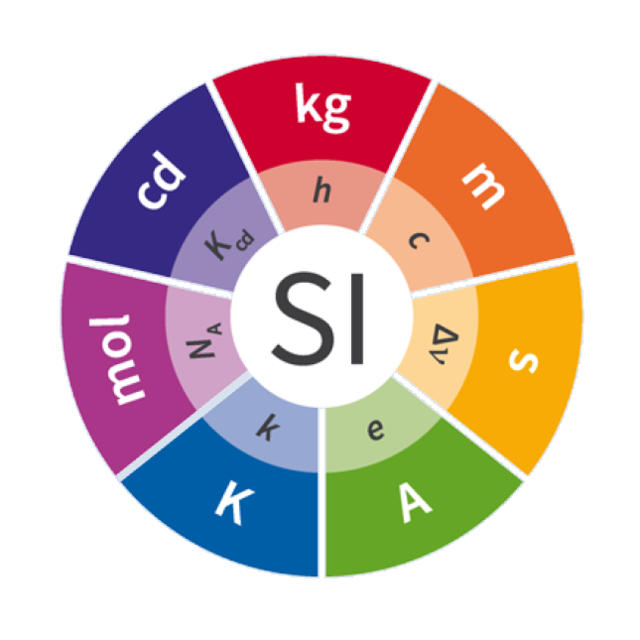
\includegraphics[scale=0.4]{Images/Fiche_Methode1/SI_Logo_with_defining_constants.png}
    \caption{Logo du système SI. }
    \label{fig:Syteme_SI}
\end{figure}
\begin{table}[!h]
    \centering
    \begin{tabularx}{\textwidth}{| X | X | c | X |}  \hline
Grandeur physique & Unité SI & Symbole de l'unité & Appareil de mesure \\
\hline
Masse & kilogramme & kg & balance \\
Temps & seconde & s & chronomètre \\
Longueur & mètre & m & règle \\
Température & kelvin & K & thermomètre \\
Intensité électrique & ampère & A & ampèremètre \\
Quantité de matière & mole & mol & balance\\
Intensité lumineuse & candela & cd & luxmètre \\
\hline
\end{tabularx}
    \caption{Tableau des unités du SI et les appareils de mesure associés.}
    \label{tab:SI}
\end{table}
\importantbox{Nous utilisons courament d'autres unités qui nous paraissent bien plus pratiques dans leur utilisation. Par exemple, nous utilisons plus facilement les degrés celsius $^\circ$C pour la température ou encore les tailles XS, S, M, L, ... pour les vêtements (même si la relation entre ces dernières \og unités \fg et les unités du SI semble très obscure...).}


\subsection{Préfixes des unités.}
Il est très souvent utile et agréable de remplacer l’écriture scientifique d’un nombre par \textbf{un nombre écrit sans puissance de 10 suivi d'un multiple ou sous-multiple de l'unité du nombre}.
\begin{table}[!h]
    \centering
    \begin{tabularx}{\linewidth}{|c|c|c|}
    \hline
    Multiple ou sous-multiple & Facteur par lequel l'unité est multipliée & Exemple typique \\ 
    \hline 
    Multiple & 1 000 000 000 000 = $10^{12}$ & Téraoctet (To) \\
    \hline
    Multiple & 1 000 000 000 = $10^{9}$ & \\
    \hline
    Multiple & 1 000 000 = $10^{6}$ & \\
    \hline
    Multiple & 1 000 = $10^{3}$ & \\
    \hline
    Multiple & 100 = $10^{2}$ & \\
    \hline
    Multiple & 10 = $10^{1}$ &  \\
    \hline
    Sous-Multiple & 0,1 = $10^{-1}$ &  \\
    \hline
    Sous-Multiple & 0, 01 = $10^{-2}$ &  \\
    \hline
    Sous-Multiple & 0, 001 = $10^{-3}$ &  \\
    
    \hline
    Sous-Multiple & 0, 000 001 = $10^{-6}$ & \\
    \hline
    Sous-Multiple & 0, 000 000 001 = $10^{-9}$ &  \\
    \hline
    Sous-Multiple & 0, 000 000 000 001 = $10^{-12}$ & \\
    \hline
    Sous-Multiple & 0, 000 000 000 000 001 = $10^{-15}$ & femtomètre (fm)\\
    \hline
    \end{tabularx}
    
    \caption{Tableaux des préfixes des multiples et sous multiples}
    \label{tab:chap1_multiples}
\end{table}

\section{Chiffres significatifs}

\begin{tcolorbox}
[colback=green!5!white,colframe=green!75!black,title=\textbf{Chiffre significatif}]
Lorsqu’on écrit une valeur en notation scientifique, le nombre de chiffres employés dans le facteur avant la puissance de 10 est le nombre de chiffres significatifs.\\
\end{tcolorbox}
Exemples : 
\begin{itemize}
    \item la célérité de la lumière $c$ dans le vide est :
\begin{equation*}
    c =\underbrace{2,99 792458}_{\text{9 chiffres significatifs}}\times 10^8~\text{m.s}^{-1}
\end{equation*}
\item 0,002 3 possède \gap{.....} chiffres significatifs car il s'écrit : 
\end{itemize}

\begin{tcolorbox}[colback=red!5!white,colframe=red!75!black,title=Règles à retenir sur les chiffres significatifs]
Le résultat d'une somme, différence, produit ou quotient est écrit avec \textbf{le plus petit nombre de chiffres signifcatifs présents dans les grandeurs dans son calcul}.
\newline
\newline
\textit{Exemple : } Calculer le temps $\Delta t$ pour que la lumière parcourt la distance Terre-Soleil $d=150\times 10^{6}$~km. Attention à mettre les grandeurs dans les bonnes unités.
\newline
\newline
\newline
\newline
\newline
\newline
\end{tcolorbox}


\section{Rédaction d'un calcul}
La réponse à une question demandant un calcul ne se résume pas l'invocation simple d'une formule non commentée et un résultat sans unité (à part bien sûr si le résultat attendu est sans unité). A chaque étape, on doit répondre de manière argumentée et présentable un calcul. Prenons l'exemple suivant : 

\begin{mdframed}[style=autreexo]
\textbf{\bsc{Exercice} - Distance Paris-Brest en train}\\
 Un TGV roule à une vitesse de l'ordre de $3,0\times 10^{2}$~km/h en France. La distance entre Paris et Brest est de 580 km.
\begin{enumerate}
\item En combien de temps une voiture roulant en moyenne à $100$~km/h effectue-t-elle ce trajet ?
\item Et un TGV ?
\end{enumerate}
\end{mdframed}

\begin{minipage}{0.5\textwidth}
    \begin{tcolorbox}[colback=red!5!white,colframe=red!75!black,title=\textbf{Mauvaise rédaction : }]
    \textbf{1)} 5,80 \\
    \textbf{2)} 1,93333333\\
    \end{tcolorbox}
\end{minipage}
\begin{minipage}{0.5\textwidth}
    \begin{tcolorbox}[colback=green!5!white,colframe=green!75!black,title=\textbf{Bonne rédaction : }]
    \textbf{1)} Le temps de parcours est donné par la formule $\Delta t=\frac{d}{v}$ avec $d$ la distance Paris-Brest et $v$ la vitesse de la voiture. Avec les données de l'énoncé, on obtient un temps de parcourt pour la voiture de :
    \begin{equation*}
        \Delta t = \frac{580}{100} = 5,8~\text{h}
    \end{equation*}
    \textbf{2)} En utilisant la même formule que la question précédente, on obtient un temps de parcourt pour le TGV de :
     \begin{equation*}
        \Delta t = \frac{580}{3,0\times 10^2} = 1,9~\text{h}
    \end{equation*}
    \end{tcolorbox}
\end{minipage}


\section{Règles de sécurité en TP de chimie}
\subsection{Les règles de sécurité}
\begin{tcolorbox}[colback=red!5!white,colframe=red!75!black,title=\textbf{En TP de chimie :}]
\vspace{10cm}
\end{tcolorbox}

\subsection{Les pictogrammes de sécurité et EPI}
\begin{figure}[!h]
    \centering
    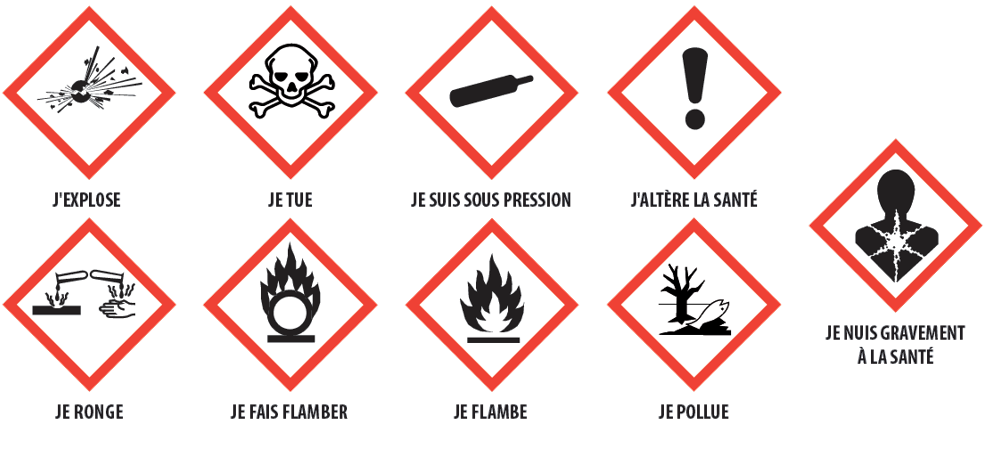
\includegraphics[scale=1]{Images/Fiche_Methode1/Pictogrammes.png}
    \caption{Pictogrammes de sécurité}
    \label{fig:enter-label}
\end{figure}

\begin{figure}[!h]
    \centering
    
\includegraphics[scale=0.9]{Images/Fiche_Methode1/picto_gant_blouse_lunette.jpg}
    \caption{Logo des \'{E}quipements de Protection Individuelle (EPI)}
    \label{fig:enter-label}
\end{figure}

\importantbox{Si vous avez un doute concernant un produit non étiquetté, il ne faut pas hésiter à regarder sa fiche de données de sécurité sur le site de l'INRS (Institut National de Recherche et de Sécurité) : \url{https://www.inrs.fr/publications/bdd/fichetox.html}}

\underline{\textbf{Exemple :}}
\begin{figure}[!h]
    \centering
    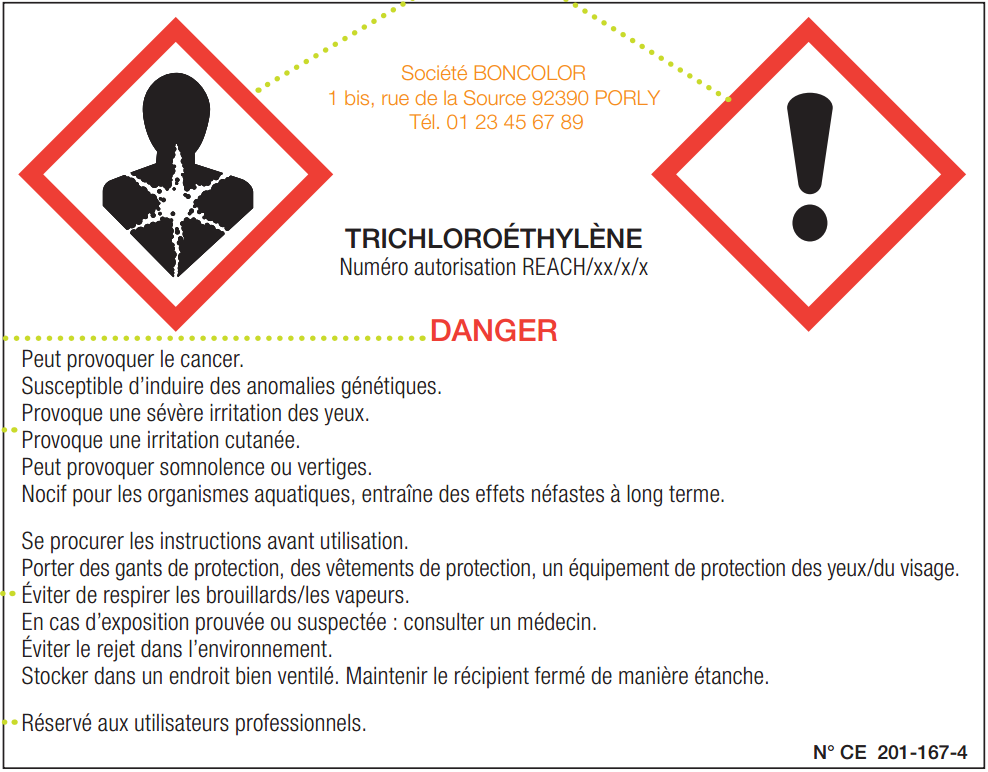
\includegraphics[scale=0.7]{Images/Fiche_Methode1/Exemple_fiche_toxico.png}
    \caption{Exemple d'une fiche de données de sécurité sur)àoi le site de l'INRS.}
    \label{fig:enter-label}
\end{figure}

